% Slides for the 2026-10-30 chat with abhi shelat and Matteo Frigo.
% Build: pdflatex longfellow-chat.tex (twice). Every number traces to
% research/dossier.md, Internship2027/reference/nvidia-fellowship/own-shield.md,
% FIPS 204, or the Falcon round-3 specification (Alg. 3, Alg. 16).
% Structure (2026-10-28 grilling): me -> my projects -> my reading of Longfellow
% -> what I could do next -> questions -> the pool ask. No competitors, no OPT.
\documentclass[aspectratio=169,11pt]{beamer}
\usetheme[progressbar=frametitle,numbering=fraction]{metropolis}
\usepackage{booktabs}
\usepackage{pgfplots}
\usetikzlibrary{positioning}
\pgfplotsset{compat=1.18}
\usepackage{xcolor}
\definecolor{accent}{HTML}{8A1C1C}
\definecolor{okgreen}{HTML}{1F6B3A}
\setbeamercolor{alerted text}{fg=accent}
\setbeamercolor{progress bar}{fg=accent}
\newcommand{\src}[1]{\par\vfill{\scriptsize\color{gray}#1}}

\title{Threshold Post-Quantum Signing,\\and the Holder Side with Longfellow}
\subtitle{A short conversation deck}
\author{Changqi Sun\\{\small PhD student, Virginia Tech (advisor: Thang Hoang)}}
\date{October 30, 2026}

\begin{document}

\maketitle

\begin{frame}{About me}
\begin{itemize}
  \item Fourth-year PhD student at Virginia Tech, applied cryptography; graduating 2028.
  \item Main line: \textbf{threshold signing for lattice signatures}, so that no single server
        holds the key and the output is a \alert{standard signature}.
  \begin{itemize}
    \item \textbf{SHIELD} (IEEE S\&P 2026, co-first author): threshold ML-DSA.
    \item \textbf{FLOCK} (first author, under submission): Falcon-compatible threshold signatures.
  \end{itemize}
  \item Also ORAM: \textbf{HERO} (first author, under review), distributed ORAM with an untrusted helper.
\end{itemize}
\vspace{.4em}
\textit{Common thread: compute and prove things about \alert{unmodified standard signatures}.}
\end{frame}

\begin{frame}{SHIELD: unmodified ML-DSA signing inside MPC (online, ML-DSA-44)}
\begin{columns}[T]
\column{.5\textwidth}
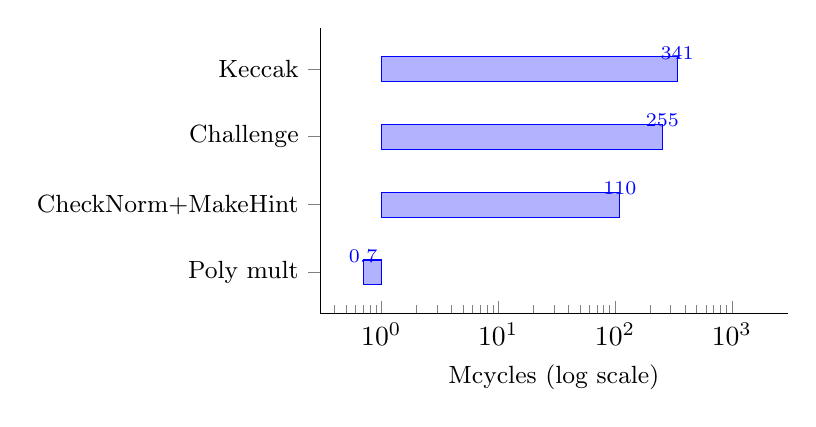
\begin{tikzpicture}
\begin{axis}[xbar, width=0.62\linewidth, height=5.2cm, xmode=log, log basis x=10,
  xmin=0.3, xmax=3000, point meta=rawx, symbolic y coords={Poly mult,CheckNorm+MakeHint,Challenge,Keccak},
  ytick=data, yticklabel style={font=\small}, xlabel={Mcycles (log scale)}, xlabel style={font=\small},
  nodes near coords, nodes near coords style={font=\scriptsize}, bar width=9pt, enlarge y limits=0.2,
  axis lines*=left, every axis plot/.append style={fill=accent!70, draw=accent}]
\addplot coordinates {(0.70,Poly mult) (110,CheckNorm+MakeHint) (255,Challenge) (341,Keccak)};
\end{axis}
\end{tikzpicture}
\column{.48\textwidth}
\footnotesize
\begin{itemize}
  \item $n$ servers, malicious security; output \alert{bit-identical} to FIPS 204 (NIST KATs).
  \item SPDZ + WRK17 garbled circuits, daBits to switch.
  \item NTTs are linear on shares: \alert{$<0.2\%$} of online compute; Boolean work dominates.
  \item Verilog $\to$ Yosys $\to$ Bristol; SampleInBall $890\text{K}\to355\text{K}$ gates.
\end{itemize}
\end{columns}
\src{SHIELD cost table (signing in MPC). ML-DSA-65/87: Keccak 438/597, poly 1.21/1.37 Mcycles.}
\end{frame}

\begin{frame}{FLOCK and the threshold-Falcon fixes}
\begin{columns}[T]
\column{.5\textwidth}
\textbf{FLOCK} (first author, under submission)
\begin{itemize}
  \item Falcon-compatible threshold signatures: the Falcon counterpart of SHIELD.
  \item Together: threshold signing for \alert{both lattice signatures NIST selected}.
\end{itemize}
\column{.5\textwidth}
\textbf{Before FLOCK: reproducing a CCS 2026 artifact}
\begin{itemize}
  \item Found two silent bugs: a PRG byte/element mix-up left $7/8$ of the sampler buffer
        uninitialized; a \texttt{size\_t} swallowed $-1$.
  \item Fixes merged upstream; signing $\approx 9\times$ faster.
\end{itemize}
\end{columns}
\vspace{.8em}
\textit{What this says about me: I read other people's cryptographic code closely,
and I check it against the spec.}
\end{frame}

\begin{frame}{My reading of Longfellow}
\begin{columns}[T]
\column{.55\textwidth}
\textbf{The statement}
\begin{itemize}
  \item An mdoc (ISO 18013-5) credential signed with \alert{ECDSA P-256 + SHA-256}: prove possession
        and reveal one attribute, with no change to the issuer.
\end{itemize}
\textbf{The recipe}
\begin{itemize}
  \item Run sumcheck, commit to the padded transcript, then prove ``the transcript makes the verifier accept'' with Ligero.
  \item Ligero only sees $d<20$ quadratic constraints, not the whole circuit.
\end{itemize}
\column{.45\textwidth}
\textbf{The fields}
\begin{itemize}
  \item P-256 base field: NTT in a quadratic extension, $\approx 1.5\times$ cost.
  \item SHA-256 in $\mathrm{GF}(2^{128})$, additive FFT.
  \item A random MAC links the witnesses of the two proofs.
\end{itemize}
\textbf{Today}: ECDSA prover 16.7\,ms (M4); CFRG draft; part of the PQCA.
\end{columns}
\src{Frigo \& shelat, CiC 2025 (ePrint 2024/2010); draft-irtf-cfrg-longfellow-00; IETF 126 slides.}
\end{frame}

\begin{frame}{Your ML-DSA circuit, through the lens of SHIELD}
\footnotesize
\begin{tabular}{@{}lll@{}}
\toprule
FIPS 204 Alg.\ 8 step & kind & Keccak-f (ML-DSA-44)\\
\midrule
$\hat{A}\gets\mathsf{ExpandA}(\rho)$ (SHAKE128) & hash & $\approx 96$\\
$tr\gets H(pk)$ & hash & $10$\\
$\mathsf{SampleInBall}$, $\tilde c' = H(\mu\,\|\,w_1')$ & hash & $\approx 10$\\
$\mathrm{NTT}^{-1}(\hat{A}\circ\hat z-\hat c\circ\widehat{t_1 2^d})$ & mod $q$ & --\\
$\mathsf{UseHint}$, $\|z\|_\infty<\gamma_1-\beta$ & range & --\\
\bottomrule
\end{tabular}
\vspace{.5em}
\begin{itemize}
  \item In \texttt{tests/pq/ml\_dsa}, $(\hat A, t_1, tr)$ are public inputs, so ExpandA and $H(pk)$ stay outside:
        $\approx 10$ permutations. \textbf{858\,ms} on an M4 (IETF 126).
  \item Same picture as signing in SHIELD: \alert{the lattice algebra is cheap, the hashing is not.}
  \item If the public key must be hidden: $\approx 116$ permutations, $\approx 4.5$M AND gates.
\end{itemize}
\src{FIPS 204; 16 ExpandA polynomials $\times \le 6$ SHAKE128 blocks; $pk$ = 1312 B over a 136 B rate; Keccak-f[1600] = 38{,}400 AND gates.}
\end{frame}

\begin{frame}{What comes next: from the issuer side to the holder side}
\centering
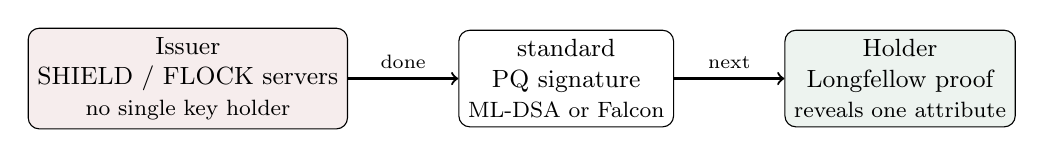
\begin{tikzpicture}[node distance=1.2cm, every node/.style={font=\small}]
\node[draw, rounded corners, align=center, fill=accent!8] (iss) {Issuer\\ SHIELD / FLOCK servers\\ \footnotesize no single key holder};
\node[draw, rounded corners, align=center, right=1.4cm of iss] (sig) {standard\\ PQ signature\\ \footnotesize ML-DSA or Falcon};
\node[draw, rounded corners, align=center, fill=okgreen!8, right=1.4cm of sig] (hold) {Holder\\ Longfellow proof\\ \footnotesize reveals one attribute};
\draw[->, thick] (iss) -- node[above, font=\scriptsize]{done} (sig);
\draw[->, thick] (sig) -- node[above, font=\scriptsize]{next} (hold);
\end{tikzpicture}
\vspace{.8em}
\begin{columns}[T]
\column{.5\textwidth}
\textbf{B. ML-DSA end to end}
\begin{itemize}\footnotesize
  \item SHIELD signs an ML-DSA credential; your existing circuit proves it.
  \item \alert{No change to the verifier or the circuit}: the signature is standard.
  \item Then: cost of the whole pipeline, issuer and holder.
\end{itemize}
\column{.5\textwidth}
\textbf{F. A Falcon circuit for Longfellow}
\begin{itemize}\footnotesize
  \item FLOCK signs Falcon credentials; the holder proves possession.
  \item Falcon verification is short, and hiding the key is almost free (next slide).
\end{itemize}
\end{columns}
\end{frame}

\begin{frame}{Why Falcon is interesting for the holder side}
\begin{columns}[T]
\column{.5\textwidth}
\textbf{Falcon verify} (round-3 spec, Alg.\ 16)
\begin{enumerate}\footnotesize
  \item $c\gets\mathsf{HashToPoint}(r\,\|\,m)$: SHAKE256, 16-bit samples, keep $t<5q$.
  \item $s_2\gets\mathsf{Decompress}(s)$.
  \item $s_1\gets c-s_2 h \bmod q$ \quad ($q=12289$, $n=512$).
  \item Accept iff $\|(s_1,s_2)\|^2\le\lfloor\beta^2\rfloor$.
\end{enumerate}
\footnotesize The public key is \alert{one polynomial} $h$: nothing to expand.
\column{.5\textwidth}
\textbf{Keccak-f per verification} (my estimate)\\[.3em]
\begin{tabular}{@{}lcc@{}}
\toprule
 & key public & key hidden\\
\midrule
ML-DSA-44 & $\approx 10$ & $\approx 116$\\
Falcon-512 & $\approx 9$ & $\approx 9$\\
\bottomrule
\end{tabular}
\vspace{.5em}

\footnotesize Open questions: Decompress in the circuit or as a witness; which field
for $q=12289$ ($q-1 = 3\cdot 2^{12}$, so a 512-point negacyclic NTT exists).
\end{columns}
\src{Falcon spec v1.2 (round 3); FIPS 206 is still a draft. 512 samples $\times$ 2 B / 0.94 acceptance $\approx$ 1.1 KB over a 136 B rate.}
\end{frame}

\begin{frame}{Questions for you}
\begin{enumerate}
  \item What is next for post-quantum Longfellow: issuer-side ML-DSA in mdoc, or device binding first?
  \item What would make the ML-DSA circuit production-grade: speed, formal verification, or the spec?
  \item Is Falcon on your radar, or is ML-DSA the only PQ target for now?
  \item Where would an intern's code land: the C++ library, the Rust rewrite, or the formal side?
\end{enumerate}
\end{frame}

\begin{frame}{One more thing}
\centering
\Large I'm already in the \alert{PhD SWE intern pool}.\\[1em]
\normalsize If you think there is a fit, would you be open to\\
requesting me from the pool for your team?\\[1.2em]
\small I'm happy to send a one-page project sketch this week.
\end{frame}

\begin{frame}[standout]
Thank you!\\[.6em]
{\normalsize changqi@vt.edu \quad changqi.dpdns.org}
\end{frame}

\end{document}
